\begin{lstlisting}
p169 1 2 5 6
\end{lstlisting}
\begin{exercise}
\begin{figure}[H]
\centering
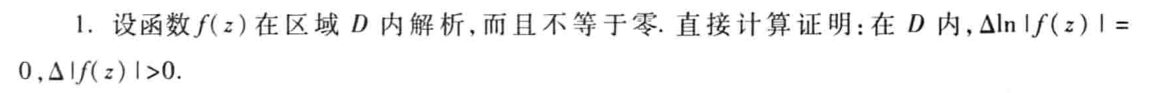
\includegraphics[width=\textwidth]{hw16-2025061511.png}
% \caption{}
\label{}
\end{figure}
\end{exercise}
显然 $f\in H(D)$, $\frac{1}{f}\in H(D)$, $D$ 单连通,故由 Rudin Theorem 13.11 可知,存在 $g\in H(D)$,使得 $f=\exp(g)$,于是
\[
\ln \lvert f(z) \rvert=\ln \lvert e^{ g(z) } \rvert=\ln \lvert e^{ \text{Re }g(z)+i\cdot \text{Im }g(z) } \rvert=\ln e^{ \text{Re }g(z) }=\text{Re }g(z)
\]
是调和函数. 记 $u\coloneqq \text{Re }g(z)$, 于是 $\Delta u=0$, 所以
\[
\Delta \lvert f(z) \rvert=(\partial _{x}^{2}+\partial _{y}^{2})(e^{ u })=e^{ u }(\partial _{x}^{2}u+\lvert \partial _{x}u \rvert ^{2}+\partial^{2}_{y}u+\lvert \partial _{y}u \rvert ^{2})=e^{ u  }(\lvert \partial _{x}u \rvert ^{2}+\lvert \partial _{y}u \rvert ^{2})\geq 0
\]
记 $g(z)=\alpha(x,y)+i\beta(x,y)$,于是由 C-R 公式:$\alpha_{x}=\beta_{y},\alpha_{y}=-\beta_{x}$. 于是 $\lvert \partial_{x}\alpha \rvert ^{2}+\lvert \partial_{y}\alpha \rvert ^{2}=\beta_{y}^{2}+\beta_{x}^{2}=\lvert g'(z) \rvert ^{2}$. 取等当且仅当 $g'\equiv0$,即 $g\equiv\text{const.}$ 也就是 $f=e^{ g }\equiv\text{const.}$

\begin{note}
不知道能不能证出来严格 $>0$.
\end{note}
\begin{exercise}
\begin{figure}[H]
\centering
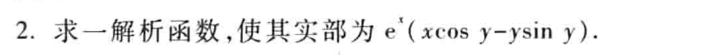
\includegraphics[width=\textwidth]{1-hw16-2025061511.png}
% \caption{}
\label{}
\end{figure}
\end{exercise}
对于解析函数 $f (z)=u (x, y)+i v(x,y)$,由 Cauchy-Riemann 方程:$u_{x}=v_{y},u_{y}=-v_{x}$. 也就是
\[
\begin{cases}
v_{y} & =e^{ x }(x+1)\cos y-e^{ x }y\sin y \\
v_{x} & =e^{ x }(x+1)\sin y +e^{ x }y\cos y
\end{cases}
\]
于是 $v(x,y)=\int v_{y}\mathrm{d}y+\phi(x)=e^x (x \sin (y)+y \cos (y))+\phi (x)$, 对 $x$ 求导得到 $v_{x}=e^{ x }(x\sin y+y\cos y+\sin y)+\phi'(x)$. 于是 $\phi'(x)=0$,故 $\phi(x)=\text{const}$. 我们可以取该解析函数为
\[
f(z)=e^{ x }(x\cos y-y\sin y)+ie^{ x }(x\sin y+y\cos y)
\]
\begin{exercise}
\begin{figure}[H]
\centering
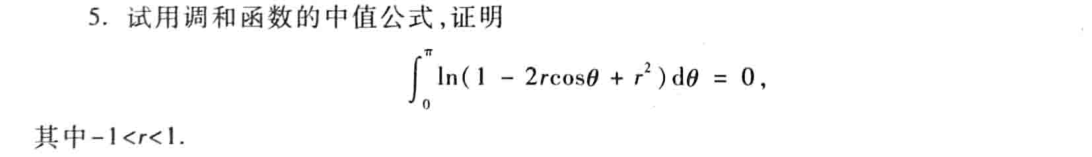
\includegraphics[width=\textwidth]{2-hw16-2025061511.png}
% \caption{}
\label{}
\end{figure}
\end{exercise}
由对称性,只需要证明
\[
\frac{1}{2\pi}\int_{0}^{2\pi}\ln (1-2r\cos\theta+r^{2}) \, \mathrm{d}\theta=0
\]
下面说明 $f(z)=\ln(1-2\text{Re }z+\lvert z^{2} \rvert)=\ln(1-2x+x^{2}+y^{2})=\ln((x-1)^{2}+y^{2})$ 是调和函数 (由于 $\lvert r \rvert<1$,该函数良好定义),直接求导得到
\[
\partial _{x}^{2}f(z)=\frac{2y^{2}-2(x-1)^{2}}{[(x-1)^{2}+y^{2}]^{2}},\quad \partial _{y}^{2}f(z)=\frac{2(x-1)^{2}-2y^{2}}{[(x-1)^{2}+y^{2}]^{2}}
\]
于是 $\Delta f(z)=0$, 故由调和函数的平均值公式
\[
f(0)=\frac{1}{2\pi}\int_{0}^{2\pi} f(re^{ i\theta }) \, \mathrm{d}\theta
\]
其中 $f(0)=\ln1=0$,$\frac{1}{2\pi}\int_{0}^{2\pi} f(re^{ i\theta }) \, \mathrm{d}\theta=\frac{1}{2\pi}\int_{0}^{2\pi} \ln(1-2r\cos\theta+r^{2}) \, \mathrm{d}\theta$. 于是
\[
\int_{0}^{\pi} \ln(1-2r\cos\theta+r^{2}) \, \mathrm{d}\theta=0
\]
\begin{exercise}
\begin{figure}[H]
\centering
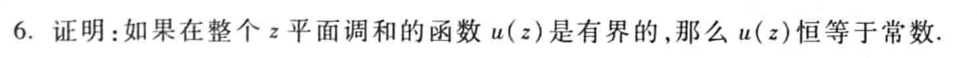
\includegraphics[width=\textwidth]{3-hw16-2025061511.png}
% \caption{}
\label{}
\end{figure}
\end{exercise}
\begin{proof}
利用平均值公式可知:$\lvert \partial_{x}u(z) \rvert\leq\frac{n}{r}\max_{\overline{B}_{r}(z)}\lvert u \rvert,\lvert \partial_{y}u(z) \rvert\leq\frac{n}{r}\max_{\overline{B}_{r}(z)}\lvert u \rvert$. 令 $r\to \infty$,就有 $\lvert \partial_{x}u \rvert=\lvert \partial_{y}u \rvert=0$,故 $u(z)$ 恒为常数.
\end{proof}
\begin{figure}[H]
\centering
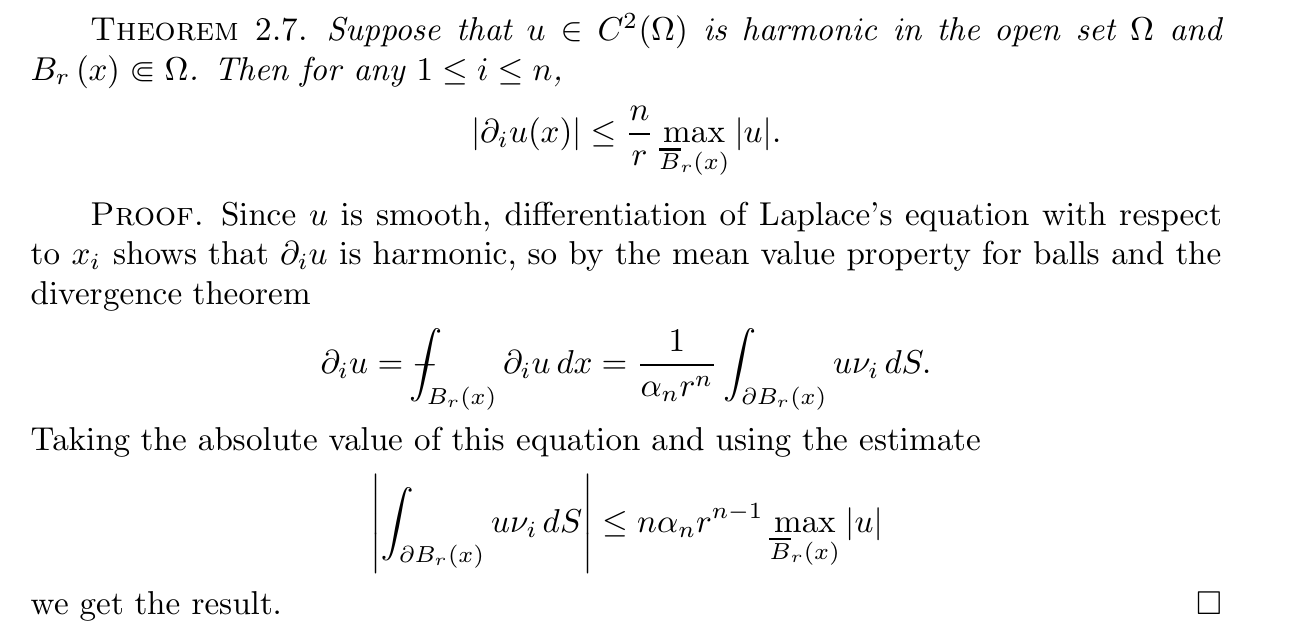
\includegraphics[width=\textwidth]{4-hw16-2025061515.png}
% \caption{}
\label{}
\end{figure}
\begin{figure}[H]
\centering
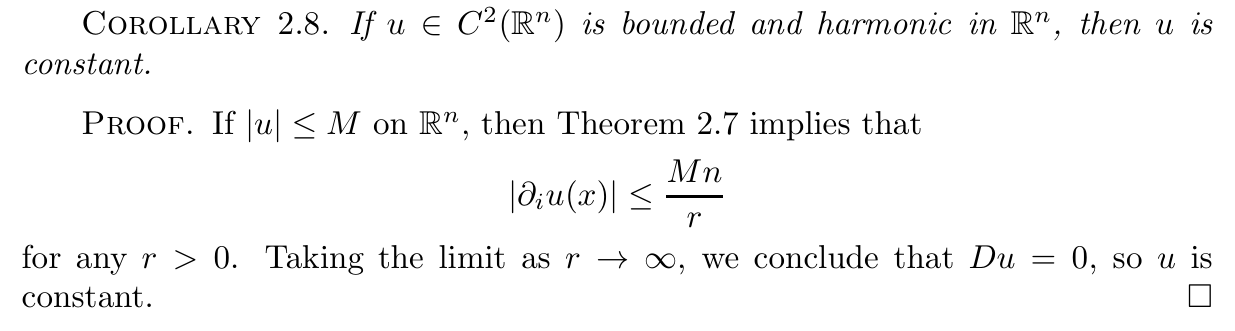
\includegraphics[width=\textwidth]{5-hw16-2025061515.png}
% \caption{}
\label{}
\end{figure}

更强的,我们证明命题在 $u$ 仅为上调和函数 ($\Delta u\geq0$) 的情况下依然成立. 这就是 2025 丘赛分析赛道第 3 题.

定义 $M(r)=\max_{\lvert z \rvert=r}u(z)$,任意给定 $0<r_1<r_2<\infty$,在区域 $\{ z\in \mathbb{C}:r_1<\lvert z \rvert<r_2 \}$ 内,断言 $\ln M(r)$ 是下凸函数. 定义
\[
h(z)=\frac{M(r_1)(\ln r_2-\ln \lvert z \rvert )+M(r_2)(\ln \lvert z \rvert -\ln r_1)}{\ln r_2-\ln r_1},\qquad \forall r_1\leq \lvert z \rvert \leq r_2
\]
$h$ 是调和函数,因为 $\Delta \ln \lvert z \rvert=(\partial_{x}^{2}+\partial_{y}^{2})\left( \frac{1}{2}\ln(x^{2}+y^{2}) \right)=\frac{y^{2}-x^{2}}{(x^{2}+y^{2})^{2}}+\frac{x^{2}-y^{2}}{(x^{2}+y^{2})^{2}}=0$. 而且
\[
u(z)\leq \lvert u(z) \rvert \leq M(r_1)=h(r_1)\qquad \forall \lvert z \rvert =r_1
\]
\[
u(z)\leq \lvert u(z) \rvert \leq M(r_2)=h(r_2)\qquad \forall \lvert z \rvert =r_2
\]
利用 Rudin Theorem 17.4 可知
\[
u(z)\leq h(z)\qquad \forall r_1\leq \lvert z \rvert \leq r_2
\]
于是对于任意 $r\in[r_1,r_2]$,我们有
\begin{equation}
M(r)\leq \frac{M(r_1)(\ln r_2-\ln r )+M(r_2)(\ln r -\ln r_1)}{\ln r_2-\ln r_1}
\label{cf008d}
\end{equation}

由于 $u$ 有上界,所以我们可以在 \cref{cf008d} 中令 $r_2\to \infty$,得到
\[
M(r)\leq M(r_1)\qquad \forall r\geq r_1
\]
也可以在 \cref{cf008d} 中令 $r_1\to0^{+}$,得到
\[
M(r)\leq M(r_2)\qquad \forall r\leq r_2
\]
由 $r_1,r_2$ 的任意性 (这里 $r_1,r_2$ 是独立的,不再有大小关系),我们知道 $M(r)$ 为常数. 考虑任意 $\mathbb{C}$ 内开区域 $G$,利用上调和函数的强极值原理,我们知道 $u$ 在 $G$ 内部取到极大值,于是 $u$ 为常数.

接下来给出 Rudin Theorem 17.4 和上调和函数的强极值原理的证明

\begin{figure}[H]
\centering
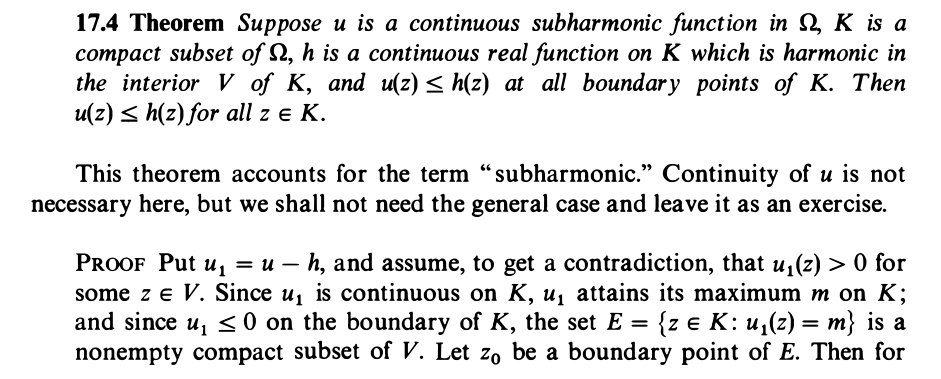
\includegraphics[width=\textwidth]{hw16-2025061515.png}
% \caption{}
\label{}
\end{figure}
\begin{figure}[H]
\centering
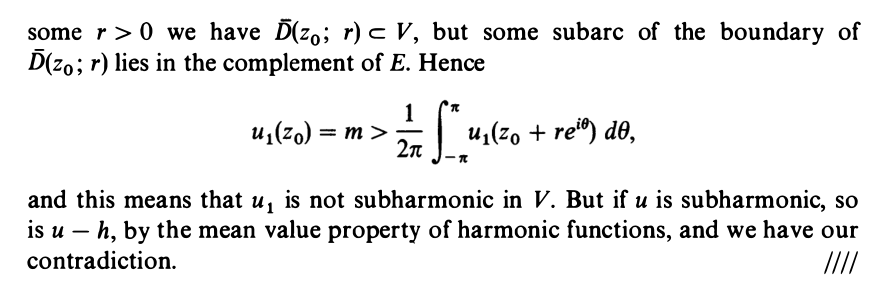
\includegraphics[width=\textwidth]{1-hw16-2025061515.png}
% \caption{}
\label{}
\end{figure}

上调和函数的强极值原理:

先叙述上调和函数的平均值公式:
\begin{figure}[H]
\centering
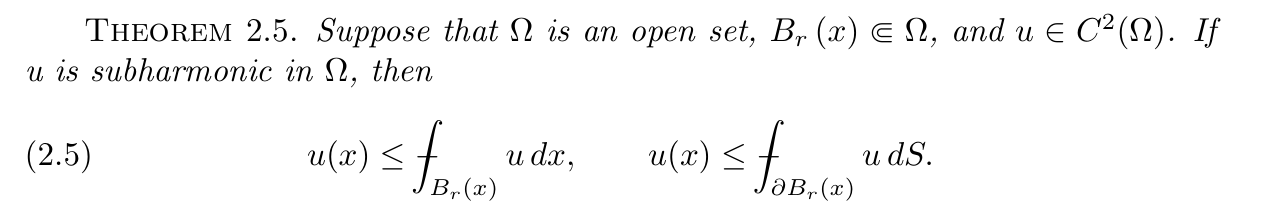
\includegraphics[width=\textwidth]{3-hw16-2025061515.png}
% \caption{}
\label{}
\end{figure}

\begin{figure}[H]
\centering
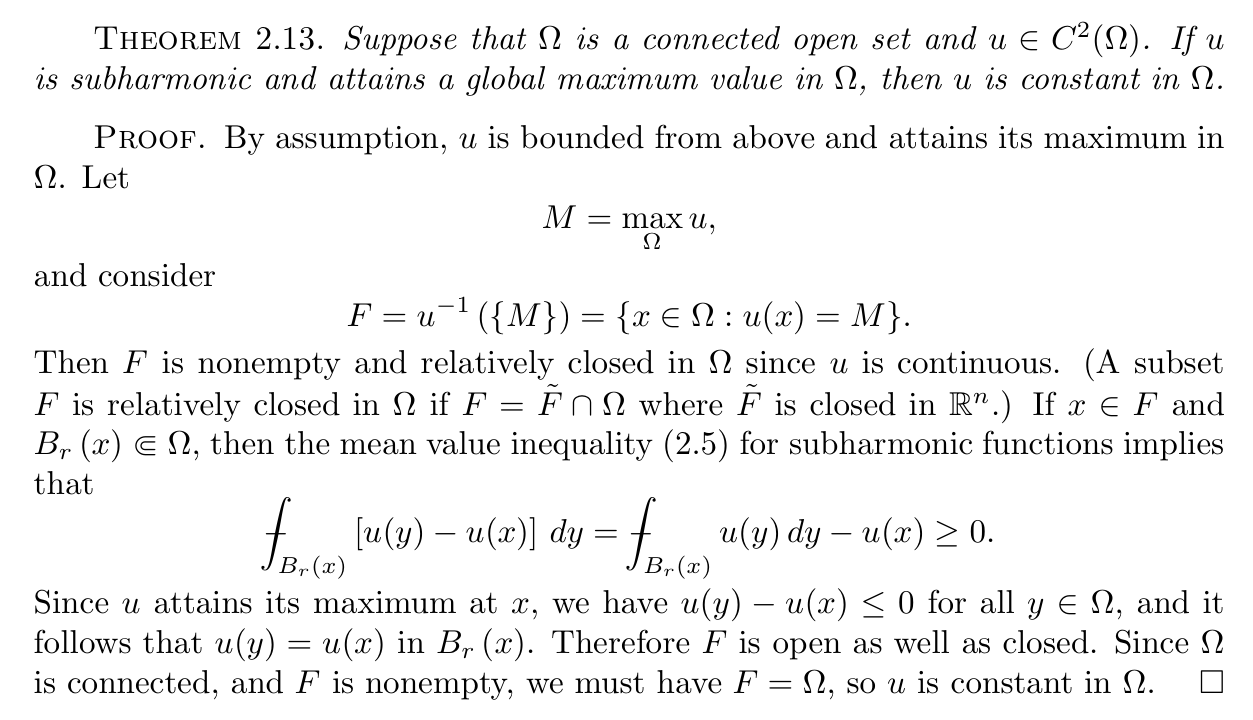
\includegraphics[width=\textwidth]{2-hw16-2025061515.png}
% \caption{}
\label{}
\end{figure}
